% ****** Start of file thzsamp.tex ******
% Complie are as follows:
%
%  1)  pdflatex thztemplate.tex
%  2)  bibtex thztemplate
%  3)  pdflatex thztemplate.tex
%  4)  pdflatex thztemplate.tex
%
\documentclass[aps,prl,twocolumn,amsmath,amssymb]{revtex4}
%\documentclass[preprint,showpacs,preprintnumbers,amsmath,amssymb]{revtex4}
\usepackage{graphicx,amsmath,epstopdf}
%\addtolength{\topmargin}{-1cm}
%\addtolength{\textheight}{4cm}

\begin{document}

\title{Probing Decoherence with Cavity Quantum Electrodynamics}% Force line breaks with \\
\author{Timothy Rose-Innes} % \email{timothy.rose-innes@ccc.ox.ac.uk} %\affiliation{}
\date{\today}% It is always \today, today,           %  but any date may be explicitly specified
\begin{abstract}
abstract
\end{abstract}
\maketitle

\section{\label{sec:level1}Introduction}

Cavity Quantum Electrodynamics (cavity QED) has proved the ideal testing ground for theories of quantum decoherence.  High quality cavities allow the interaction of the atom-field system with the external environment to be minimised and well characterised. This provides experimentalists with a model system for demonstrations quantum control. However, conversely, this also creates an opportunity to rigorously study the theories of open quantum systems and the its manifestation as quantum decoherence.
 
In cavity QED, the cavity is at its most basic a set of mirrors that can support modes of the electromagnetic field. Of principle interest are optical or microwave resonators.  “QED” or quantum electrodynamics refers to the interaction of quantum matter with those cavity modes. In this report we are concerned with two-level atoms, a physical realisation of a quantum qubit . It is also important to point out that there are many other analogous physical systems consisting of a resonator coupled to a two level system. These include superconducting qubits coupled to microwave resonators, know as “circuit QED”  and also mechanical systems coupled to cavities.  Quantum decoherence is the phenomena of an open system interacting with its environment  leading to the loss of coherences in the system.

Work in the field of Cavity QED has over the last few decades been at the forefront of testing our understanding of the quantum world and particularly quantum decoherence. Indeed it is for work in the field that Serge Haroche was jointly  awarded the 2012 noble prize for "for ground-breaking experimental methods that enable measuring and manipulation of individual quantum systems'' This report will consider three of the main experiments performed by the Haroche Group at l’Ecole Normale
Sup´erieure (ENS) that elucidate aspects of quantum decoherence; The decoherence of Schrödinger cat states, the observation of quantum jumps and finally its application in  feedback. Initially, we will review the basics of Cavity QED and the theories of open quantum systems and decoherence.

\section{\label{sec:level2}Background: Cavity QED}

Quantum oscillators are ubiquitous in the microscopic quantum world.  The quantised oscillation of light in a cavity is a prime example of such physical behaviour. The advent of High quality microwave cavities has provide an excellent opportunity to study this model system lights interaction with matter.  

The cavities utilised in such experiments consist of two spherical mirrors in a Fabry-Perot configuration. Typically the mirrors are constructed from superconducting niobium allowing for high quality factors; the quality factor is proportional to the conductivity of the mirrors surface.  Quality factors of the order 2x1010ms have been realised. The cavity is cooled to 0.8K. Typical cavity lifetimes are of order 100ms. A classical source of microwaves pumps the cavity to form low amplitude coherent states.

The cavity is open on both sides to allow atoms to pass through the setup and interact with the field. The atoms used are circular Rydberg Atoms. Rydberg atoms are excited atoms with electrons in states of  very high principle quantum number, n. Circular Rydberg atoms have maximum orbital angular momentum quantum number, $l = n +1$ and maximum magnetic quantum number $|m| = n +1$. Typically Rubidium atoms excited to levels \textbf{n = 50} and \textbf{n = 51} realise the states $|g\rangle$ and $|e\rangle$.Circular Rydberg atoms are used for a number of reasons. They have allowed dipole transitions, large dipole moments and low spontaneous emission rates with lifetimes $\tau$ = 0.1s. Furthermore the ability to selectively ionise them by applied fields allows selective setection of the $|g\rangle$ and $|e\rangle$ states.

The interaction of light and a two level atom is modelled by the Jaynes-Cummings Hamiltonian. 

\begin{align}
 H_{JC} =\frac{\hbar \Omega_0}{2} \left(\hat{a}\hat{\sigma}_+
+\hat{a}^{\dagger}\hat{\sigma}_-\right)
\label{eq:cat1}.
\end{align}

In the case of large detuning, $\delta$.

\begin{align}
H_{disp} = \hbar \chi\left(\hat{a}^{\dagger}\hat{a}\hat{\sigma}_z\right)
\label{eq:cat1}.
\end{align}

In the regime of $\delta$ of order or smaller than $\sqrt{\bar{n}} \Omega_0$ we have  $\chi = \frac{\Omega_0}{4 \sqrt{\bar{n}}}$


\section{\label{sec:level1}Background: Decoherence in Cavity QED}

\section{\label{sec:level1}Background: Experimental Setup}

\section{\label{sec:level1}Decoherence of Schroedinger Cat}

Schrödinger's famous Gedankenexperiment was formulated in order to expose what he saw as the absurdity of the Copenhagen interpreatation of quantum mechanics.  

\subsection{\label{sec:level1}Preparation of the Cat states}


We define our Schrödinger cat state as a superposition of two coherent states of light with equal probabilities but different field amplitudes. We will particular be concerned with phase cats where the coherent states in the superposition have the same amplitude $\beta_1$ but with phases differing by $\pi$

\begin{align}
|\psi_{\mathrm{cat}}\rangle = \frac{1}{\sqrt{2}} (|\beta e^{i\Phi}\rangle+|\beta e^{-i\Phi}\rangle)
\label{eq:cat1}.
\end{align}

However, this is not the whole picture; the cat must then be entangled with an atom to form the state

\begin{align}
|\psi_{\mathrm{cat}}\rangle = \frac{1}{\sqrt{2}} (|e\rangle|\beta e^{i\Phi}\rangle+|g\rangle|\beta e^{-i\Phi}\rangle)
\label{eq:cat2}.
\end{align}

The setup to meter that is sensitive to the phase shift in the atomic state superposition caused by the atoms interaction witexperimentally realise this state state is pictured in figure ~\ref{fig:Setup}. A coherent state is injected into the microwave cavity (C) using a classical pulsed source; the coherent state has an amplitude $|\beta| = \sqrt(n_{m})$ where $n_{m}$ is mean photon number. An atom from an atomic beam B are prepared in the state $g\rangle$. The atomic states $|g\rangle$ and $|e\rangle$ refer to the neighbouring circular Rydberg levels utilised as they have a long life-time and couple strongly to the microwave field.  The atoms is then passed through a low quality microwave cavity $\mathrm{R_{1}}$ transforming the state $|g\rangle \rightarrow  (|e\rangle+|g\rangle)/\sqrt{2}$. Auxiliary microwave cavities $\mathrm{R_{1}}$ and $\mathrm{R_{2}}$ together form a Ramsey interferoh the cavity. 

The cavity C is detuned slightly from the $|e\rangle \rightarrow |g\rangle$ transition by an amount $\delta$.  The dispersive interaction of the atom and the cavity leads to a phase shift $\pm\Omega/\delta^2$ of the field dependent on the state of the atom. This brings the combined atom and field state into the desired cat state in equation 1~\ref{eq:cat2}.

The second auxiliary cavity R1 applies a microwave pulse %of phase shifted from that of R1 by $\nu$
remixing the atomic states to form 

\begin{align}
|\psi_{\mathrm{cat}}\rangle = \frac{1}{2} ((|e\rangle-|g\rangle)|\beta e^{i\Phi}\rangle+(|e\rangle+|g\rangle)|\beta e^{-i\Phi}\rangle)
\label{eq:cat3}.
\end{align}

Finally the atoms are detected in the states $|e\rangle$ and $|g\rangle$ using field ionisation detectors and the field projected into  $\frac{1}{\sqrt{2}} (|\beta e^{i\Phi}\rangle \pm|\beta e^{-i\Phi}\rangle)$

\subsection{\label{sec:level1}Probing the decoherence of The Cat states}




\begin{figure}
  \centering
  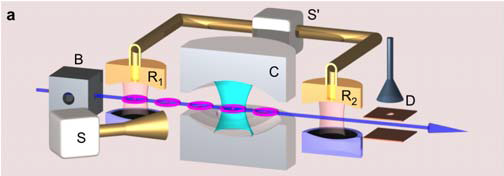
\includegraphics[width=.8\linewidth]{Figures/fig_ramsey_interf.png}
\caption{The joint spectral amplitude (JSA) of a (SPDC) biphoton state is product of two functions, the pump function, $\alpha(\omega_A,\omega_B)$ and the phase matching function, $\phi(\omega_A,\omega_B)$.}
\label{fig:Setup}
\end{figure}
Figures/UncorrelatedSHOMI.eps


\section{\label{sec:level1}Quantum Jumps}

\section{\label{sec:level1}Quantum Feedback}






\bibliography{roy}

\end{document}
